\documentclass[12pt,a4paper]{article}
\usepackage[utf8]{vietnam}
\usepackage{amsmath,amssymb,amsfonts,mathrsfs}
\usepackage[left=1.5cm,right=1.5cm,top=2cm,bottom=2cm,headheight=17pt]{geometry}
\usepackage{enumitem}
\usepackage{array}
\usepackage{graphicx}
\usepackage{fancyhdr}

\pagestyle{fancy}
\fancyhf{}
\lhead{\small\textbf{HƯỚNG TỚI THPTQG 2027}}
\rhead{\small\textit{Người biên soạn: Dương Gia Bảo}}
\rfoot{\small Trang \thepage}
\renewcommand{\headrulewidth}{0.4pt}

\begin{document}

\noindent
\begin{minipage}[t]{0.40\textwidth}
    \centering
    \textbf{HƯỚNG TỚI THPTQG 2027}\\[-2pt]
    \rule{3.2cm}{0.6pt}\\[4pt]
    \textbf{ĐỀ CHÍNH THỨC}
\end{minipage}\hfill
\begin{minipage}[t]{0.58\textwidth}
    \centering
    \textbf{ĐỀ THI KHẢO SÁT CHẤT LƯỢNG}\\
    \textbf{ĐỀ SỐ 4}\\
    \textbf{Môn thi: TOÁN}\\
    \textit{\small Thời gian làm bài: 90 phút, không kể thời gian phát đề}
\end{minipage}

\vspace{0.2cm}
\noindent
\begin{minipage}[b]{0.78\textwidth}
    \textbf{Họ và tên:}\dotfill\textbf{SBD:}\makebox[3.5cm]{\dotfill}
\end{minipage}\hfill
\begin{minipage}[b]{0.20\textwidth}
    \hfill
    \setlength{\fboxrule}{0.8pt}%
    \fbox{\begin{minipage}{2.3cm}
        \centering
        \textbf{\small Mã đề thi}\\
        \textbf{0004}
    \end{minipage}}
\end{minipage}
\vspace{0.2cm}

% ==========================================
% PHẦN I
% ==========================================
\section*{\large PHẦN I. CÂU TRẮC NGHIỆM NHIỀU PHƯƠNG ÁN LỰA CHỌN}
\textit{Thí sinh trả lời từ câu 1 đến câu 12. Mỗi câu hỏi thí sinh chỉ chọn một phương án. Mỗi câu trả lời đúng được 0,25 điểm.}

\begin{enumerate}[label=\textbf{Câu \arabic*:}, leftmargin=*]

\item Cho hàm số $y = \dfrac{x^2 - 3x + 6}{x - 1}$ có đồ thị là $(C)$. Khoảng cách giữa hai điểm cực trị $A$ và $B$ của đồ thị hàm số $(C)$ bằng
\begin{enumerate}[label=\Alph*.]
    \item $2\sqrt{5}$.
    \item $8\sqrt{2}$.
    \item $4\sqrt{5}$.
    \item $4\sqrt{2}$.
\end{enumerate}

\item Sau khi uống một liều thuốc cảm sốt, nồng độ thuốc trong máu của bệnh nhân (đơn vị: mg/L) sau $t$ giờ ($t \ge 0$) được mô hình hóa bởi hàm số:
$$C(t) = \dfrac{30t}{t^2 + 9}$$
Hỏi nồng độ thuốc cao nhất trong máu bệnh nhân đạt mức bao nhiêu mg/L?
\begin{enumerate}[label=\Alph*.]
    \item $3\text{ mg/L}$.
    \item $5\text{ mg/L}$.
    \item $6\text{ mg/L}$.
    \item $10\text{ mg/L}$.
\end{enumerate}

\item Có bao nhiêu giá trị nguyên của tham số $m \in [-10; 10]$ để bất phương trình $\log_{0{,}5}(x^2 - 4x + m) \ge -3$ nghiệm đúng với mọi số thực $x \in [1; 3]$?
\begin{enumerate}[label=\Alph*.]
    \item $4$.
    \item $5$.
    \item $7$.
    \item $6$.
\end{enumerate}

\item Để kéo dãn một sợi dây cáp thép đàn hồi một đoạn $x$ (mét) so với trạng thái tự nhiên, cần tác dụng một lực kéo biến thiên theo hàm số $F(x) = 400x + 120x^2\text{ (N)}$. Công cơ học $W = \int_0^{0{,}5} F(x) dx$ sinh ra khi kéo sợi cáp dãn từ trạng thái tự nhiên ($x = 0$) đến độ dãn $x = 0{,}5\text{ m}$ bằng
\begin{enumerate}[label=\Alph*.]
    \item $45\text{ J}$.
    \item $50\text{ J}$.
    \item $55\text{ J}$.
    \item $60\text{ J}$.
\end{enumerate}

\item Trong không gian $Oxyz$, cho điểm $A(2; 1; -3)$ và mặt phẳng $(P): 2x - 2y + z - 8 = 0$. Tọa độ hình chiếu vuông góc $H$ của điểm $A$ lên mặt phẳng $(P)$ là
\begin{enumerate}[label=\Alph*.]
    \item $H(4; -1; -2)$.
    \item $H(0; 3; -4)$.
    \item $H(2; -1; 0)$.
    \item $H(6; -3; -1)$.
\end{enumerate}

\item Khảo sát thời gian tự học mỗi tuần (đơn vị: giờ) của 50 học sinh lớp 12 thu được mẫu số liệu ghép nhóm sau:
\begin{center}
\begin{tabular}{|c|c|c|c|c|c|}
\hline
\textbf{Thời gian (giờ)} & $[5; 10)$ & $[10; 15)$ & $[15; 20)$ & $[20; 25)$ & $[25; 30)$ \\ \hline
\textbf{Số học sinh} & $8$ & $16$ & $14$ & $8$ & $4$ \\ \hline
\end{tabular}
\end{center}
Khoảng tứ phân vị $\Delta_Q = Q_3 - Q_1$ của mẫu số liệu ghép nhóm trên bằng bao nhiêu (làm tròn kết quả đến hai chữ số thập phân)?
\begin{enumerate}[label=\Alph*.]
    \item $7{,}85\text{ giờ}$.
    \item $8{,}42\text{ giờ}$.
    \item $9{,}12\text{ giờ}$.
    \item $8{,}95\text{ giờ}$.
\end{enumerate}

\item Khảo sát tại một trường học ghi nhận $65\%$ học sinh yêu thích môn Bóng đá ($A$), $50\%$ học sinh yêu thích môn Bóng rổ ($B$), và có $85\%$ học sinh yêu thích ít nhất một trong hai môn thể thao này ($A \cup B$). Chọn ngẫu nhiên một học sinh trong trường. Biết rằng học sinh đó thích môn Bóng đá, tính xác suất để học sinh đó cũng thích môn Bóng rổ (làm tròn kết quả đến hàng phần trăm).
\begin{enumerate}[label=\Alph*.]
    \item $0{,}35$.
    \item $0{,}50$.
    \item $0{,}40$.
    \item $0{,}46$.
\end{enumerate}

\item Cho hàm số $y = \dfrac{2x^2 + 3x - 1}{x + 2}$. Đường tiệm cận xiên của đồ thị hàm số tạo với hai trục tọa độ $Ox, Oy$ một tam giác có diện tích bằng
\begin{enumerate}[label=\Alph*.]
    \item $0{,}25$.
    \item $0{,}50$.
    \item $1{,}00$.
    \item $0{,}75$.
\end{enumerate}

\item Đồng vị phóng xạ I-ốt 131 dùng trong điều trị y tế có chu kỳ bán rã là 8 ngày (cứ sau 8 ngày, lượng chất phóng xạ giảm đi một nửa). Ban đầu có một mẫu chứa $200\text{ mg}$ I-ốt 131. Sau 32 ngày liên tục, khối lượng I-ốt 131 còn lại trong mẫu bằng
\begin{enumerate}[label=\Alph*.]
    \item $25\text{ mg}$.
    \item $12{,}5\text{ mg}$.
    \item $6{,}25\text{ mg}$.
    \item $50\text{ mg}$.
\end{enumerate}

\item Trong không gian $Oxyz$, cho mặt cầu $(S): (x - 1)^2 + (y - 2)^2 + (z + 1)^2 = 9$ và điểm $A(4; 6; 11)$. Khoảng cách ngắn nhất từ điểm $A$ đến một điểm $M$ bất kỳ thuộc mặt cầu $(S)$ bằng
\begin{enumerate}[label=\Alph*.]
    \item $7$.
    \item $16$.
    \item $10$.
    \item $13$.
\end{enumerate}

\item Cho hình phẳng $(H)$ giới hạn bởi đồ thị hàm số $y = \sqrt{x \ln x}$, trục hoành và đường thẳng $x = e$. Thể tích $V$ của khối tròn xoay thu được khi quay hình phẳng $(H)$ xung quanh trục $Ox$ bằng
\begin{enumerate}[label=\Alph*.]
    \item $V = \dfrac{\pi(e^2 + 1)}{4}$.
    \item $V = \dfrac{\pi(e^2 - 1)}{4}$.
    \item $V = \dfrac{\pi(e^2 + 1)}{2}$.
    \item $V = \dfrac{\pi(e^2 - 1)}{2}$.
\end{enumerate}

\item Có bao nhiêu giá trị nguyên của tham số $m \in [-10; 10]$ để hàm số $y = x^3 - 3mx^2 + 3(m^2 - 1)x + 2$ có hai điểm cực trị $x_1, x_2$ thỏa mãn điều kiện $x_1^2 + x_2^2 = 10$?
\begin{enumerate}[label=\Alph*.]
    \item $0$.
    \item $1$.
    \item $4$.
    \item $2$.
\end{enumerate}

\end{enumerate}

% ==========================================
% PHẦN II
% ==========================================
\section*{PHẦN II. CÂU TRẮC NGHIỆM ĐÚNG/SAI}
\textit{Thí sinh trả lời từ câu 1 đến câu 4. Trong mỗi ý a), b), c), d) ở mỗi câu, thí sinh chọn Đúng hoặc Sai.}

\begin{enumerate}[label=\textbf{Câu \arabic*:}, leftmargin=*]

\item Một xưởng may gia công sản xuất $x$ trăm bộ quần áo bảo hộ lao động mỗi tháng ($0 < x \le 30$). Chi phí sản xuất $x$ trăm bộ quần áo là $C(x) = x^3 - 18x^2 + 120x + 80$ (triệu đồng). Giá bán mỗi trăm bộ quần áo phụ thuộc vào số lượng sản xuất theo hàm giá $p(x) = 180 - 6x$ (triệu đồng/trăm bộ).
\begin{center}
    
\includegraphics[width=0.42\linewidth,height=3.2cm,keepaspectratio]{images/phan2_cau1_maybaoholaodong.jpg}
\end{center}
\begin{enumerate}[label=\alph*)]
    \item Tổng doanh thu thu được khi bán hết $x$ trăm bộ quần áo là $R(x) = 180x - 6x^2$ (triệu đồng).
    \item Hàm lợi nhuận hàng tháng của xưởng may được xác định bởi $L(x) = -x^3 + 12x^2 + 60x + 80$ (triệu đồng).
    \item Để đạt được lợi nhuận lớn nhất, xưởng may cần sản xuất và bán $10$ trăm bộ ($1.000$ bộ) quần áo bảo hộ mỗi tháng.
    \item Mức lợi nhuận hàng tháng lớn nhất mà xưởng may có thể đạt được là $720$ triệu đồng.
\end{enumerate}

\item Một ô tô điện đang di chuyển trên đường thử nghiệm với vận tốc $v_0 = 27\text{ m/s}$ thì người lái xe bắt đầu đạp phanh. Kể từ thời điểm $t = 0$ (giây), gia tốc hãm phanh biến thiên theo thời gian theo hàm số $a(t) = -1{,}5t\text{ (m/s}^2\text{)}$.

\begin{enumerate}[label=\alph*)]
    \item Sau $2$ giây kể từ khi đạp phanh, vận tốc của ô tô điện bằng $24\text{ m/s}$.
    \item Gia tốc hãm phanh của xe tại thời điểm $t = 4$ giây có độ lớn bằng $5\text{ m/s}^2$.
    \item Kể từ lúc bắt đầu đạp phanh, sau đúng $6$ giây thì chiếc xe điện dừng lại hoàn toàn.
    \item Quãng đường ô tô điện di chuyển được từ lúc bắt đầu đạp phanh cho đến khi dừng hẳn vượt quá $110\text{ m}$.
\end{enumerate}

\item Trong một đợt tầm soát vi-rút cúm gia cầm tại vùng chăn nuôi tập trung, tỉ lệ gia cầm nhiễm vi-rút là $5\%$. Một kit thử sinh học được áp dụng có độ nhạy $96\%$ (gia cầm nhiễm vi-rút có xác suất thử ra kết quả dương tính là $96\%$) và độ đặc hiệu $90\%$ (gia cầm không nhiễm vi-rút có xác suất thử ra kết quả âm tính là $90\%$). Chọn ngẫu nhiên một con gia cầm trong vùng để xét nghiệm.
\begin{enumerate}[label=\alph*)]
    \item Xác suất con gia cầm được chọn không bị nhiễm vi-rút cúm gia cầm là $0{,}95$.
    \item Xác suất một con gia cầm không bị nhiễm vi-rút nhưng kit thử lại báo kết quả dương tính giả bằng $0{,}10$.
    \item Xác suất để một con gia cầm được chọn ngẫu nhiên có kết quả xét nghiệm dương tính bằng $0{,}143$.
    \item Nếu con gia cầm được chọn có kết quả xét nghiệm dương tính, xác suất để con gia cầm đó thực sự bị nhiễm vi-rút lớn hơn $35\%$.
\end{enumerate}

\item \begin{minipage}[t]{0.55\linewidth}
Một kết cấu mái che vòm thép của sân thi đấu tennis có dạng hình chóp $S.ABCD$ đặt trong hệ tọa độ $Oxyz$ (đơn vị đo trên các trục là mét). Đỉnh vòm $S$ có tọa độ $S(4; 5; 8)$, mặt sàn nằm trên mặt phẳng $z = 0$ với 4 chân cột là $A(0; 0; 0)$, $B(8; 0; 0)$, $C(8; 10; 0)$, $D(0; 10; 0)$. Bốn thanh cáp chống chịu $SA, SB, SC, SD$ nối từ đỉnh $S$ xuống 4 chân cột.
\begin{enumerate}[label=\alph*)]
    \item Tọa độ hình chiếu vuông góc $H$ của đỉnh vòm $S$ lên mặt phẳng sàn $(ABCD)$ là $H(4; 5; 0)$.
    \item Độ dài của thanh cáp $SA$ bằng $\sqrt{105}\text{ m}$.
    \item Tọa độ trọng tâm $G$ của tam giác đáy $ABC$ là $G\left(\dfrac{16}{3}; \dfrac{10}{3}; 0\right)$.
    \item Góc nghiêng tạo bởi thanh cáp $SA$ và mặt sàn $z = 0$ nhỏ hơn $45^\circ$.
\end{enumerate}
\end{minipage}\hfill
\begin{minipage}[t]{0.42\linewidth}
\vspace{-0.7\baselineskip}
\centering
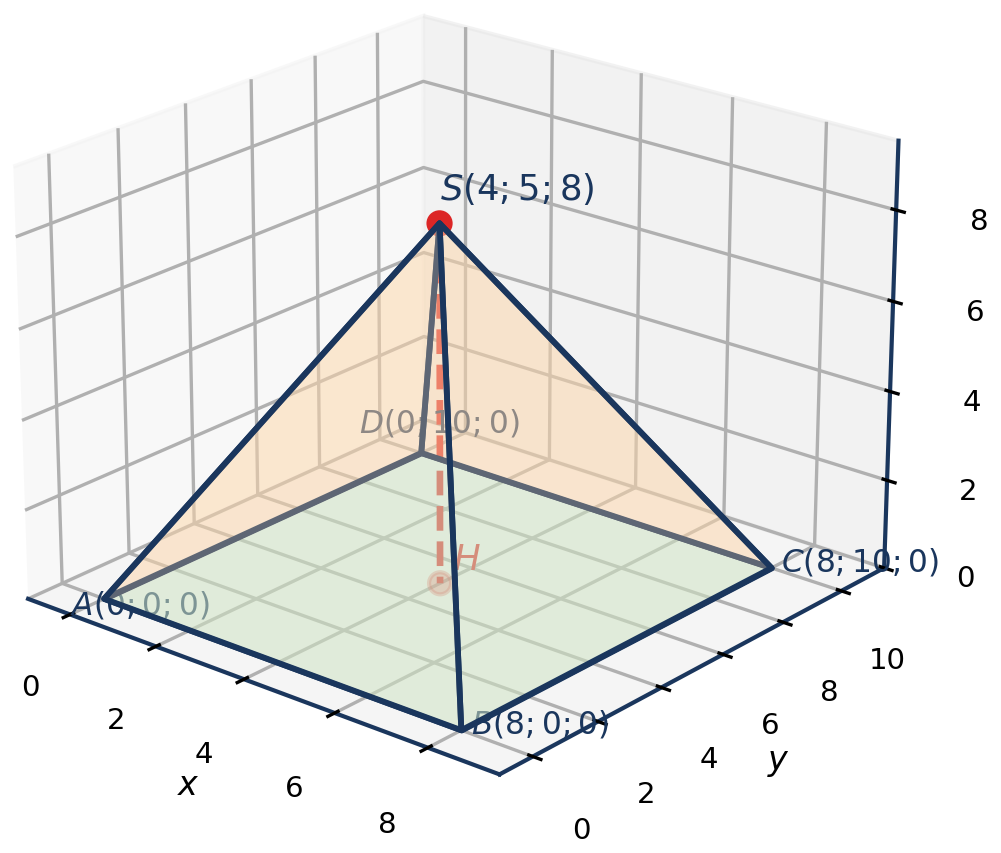
\includegraphics[width=\linewidth]{images/phan2_cau4_maiche_oxyz.png}
\end{minipage}

\end{enumerate}

% ==========================================
% PHẦN III
% ==========================================
\section*{PHẦN III. CÂU TRẮC NGHIỆM TRẢ LỜI NGẮN}
\textit{Thí sinh trả lời từ câu 1 đến câu 6. Điền đáp số theo quy chuẩn làm tròn được nêu trong từng câu.}

\begin{enumerate}[label=\textbf{Câu \arabic*:}, leftmargin=*]

\item \begin{minipage}[t]{0.57\linewidth}
Bác Hùng muốn làm một chiếc thùng đựng rác công nghiệp bằng tôn không nắp dạng hình hộp chữ nhật có đáy là hình vuông cạnh $x\text{ (m)}$ và chiều cao $h\text{ (m)}$. Thể tích của chiếc thùng rác được ấn định bằng $0{,}162\text{ m}^3$. Bác Hùng tính toán chi phí tôn làm đáy là $150.000\text{ đồng/m}^2$ và chi phí tôn làm 4 mặt bên xung quanh là $100.000\text{ đồng/m}^2$. Tìm giá trị của $x$ (m) để tổng chi phí mua tôn làm thùng rác đạt giá trị nhỏ nhất (làm tròn kết quả đến hàng phần mười của mét).
\end{minipage}\hfill
\begin{minipage}[t]{0.40\linewidth}
\vspace{-0.7\baselineskip}
\centering
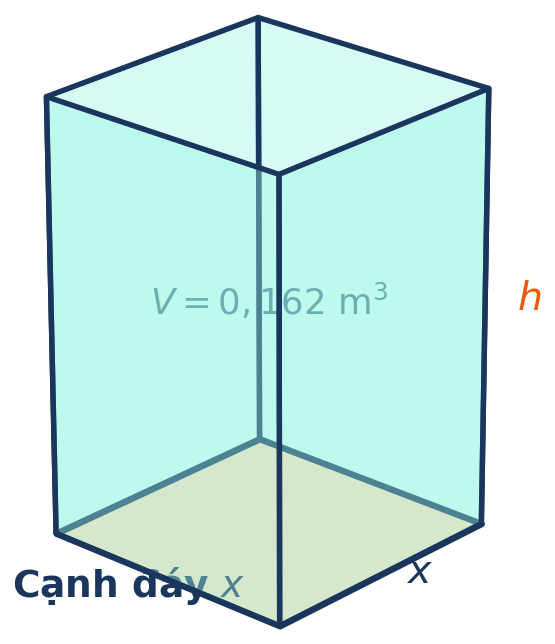
\includegraphics[width=0.92\linewidth]{images/phan3_cau1_thungrac_3d.png}
\end{minipage}

\item Chị Mai gửi cố định vào đầu mỗi tháng $10$ triệu đồng vào ngân hàng theo hình thức tiết kiệm tích lũy định kỳ với lãi suất $0{,}6\%$/tháng (lãi nhập gốc hàng tháng). Chị Mai muốn tích lũy tổng số tiền cả gốc và lãi đạt tối thiểu $500$ triệu đồng để chuẩn bị mở cửa hàng kinh doanh. Hỏi chị Mai cần gửi tiền liên tục trong ít nhất bao nhiêu tháng?
\begin{center}
    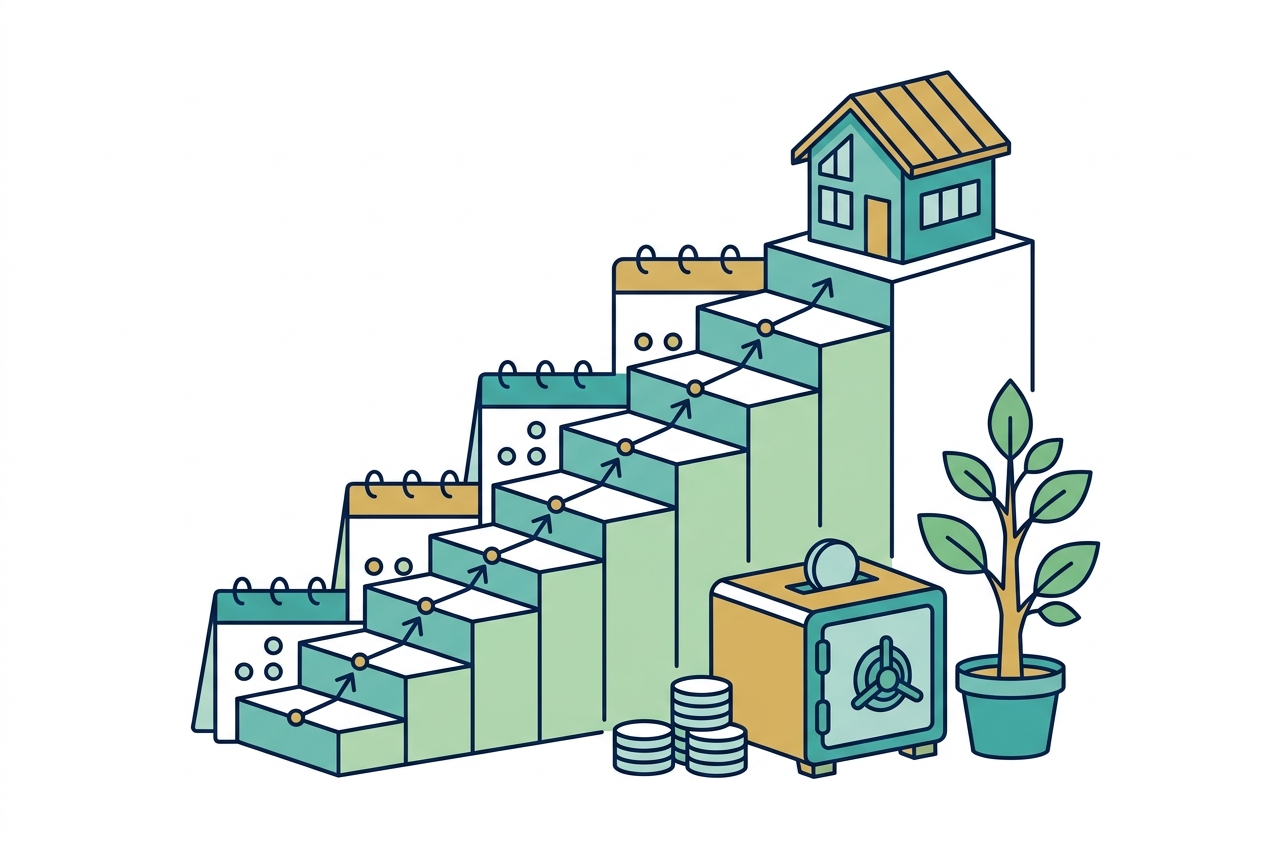
\includegraphics[width=0.42\linewidth,height=3.2cm,keepaspectratio]{images/phan3_cau2_tietkiem.jpg}
\end{center}

\item \begin{minipage}[t]{0.55\linewidth}
Một đài ra-đa kiểm soát hàng không đặt tại vị trí gốc tọa độ $O(0; 0; 0)$ trong hệ tọa độ $Oxyz$ (đơn vị trên các trục là km). Một chiếc máy bay thương mại đang trong quá trình bay chuyển động thẳng đều đi qua hai điểm mốc $A(3; 2; 4)$ và $B(7; 6; 8)$. Tìm khoảng cách ngắn nhất từ đài ra-đa $O$ đến đường bay của máy bay (làm tròn kết quả đến hàng phần mười của km).
\end{minipage}\hfill
\begin{minipage}[t]{0.42\linewidth}
\vspace{-0.7\baselineskip}
\centering
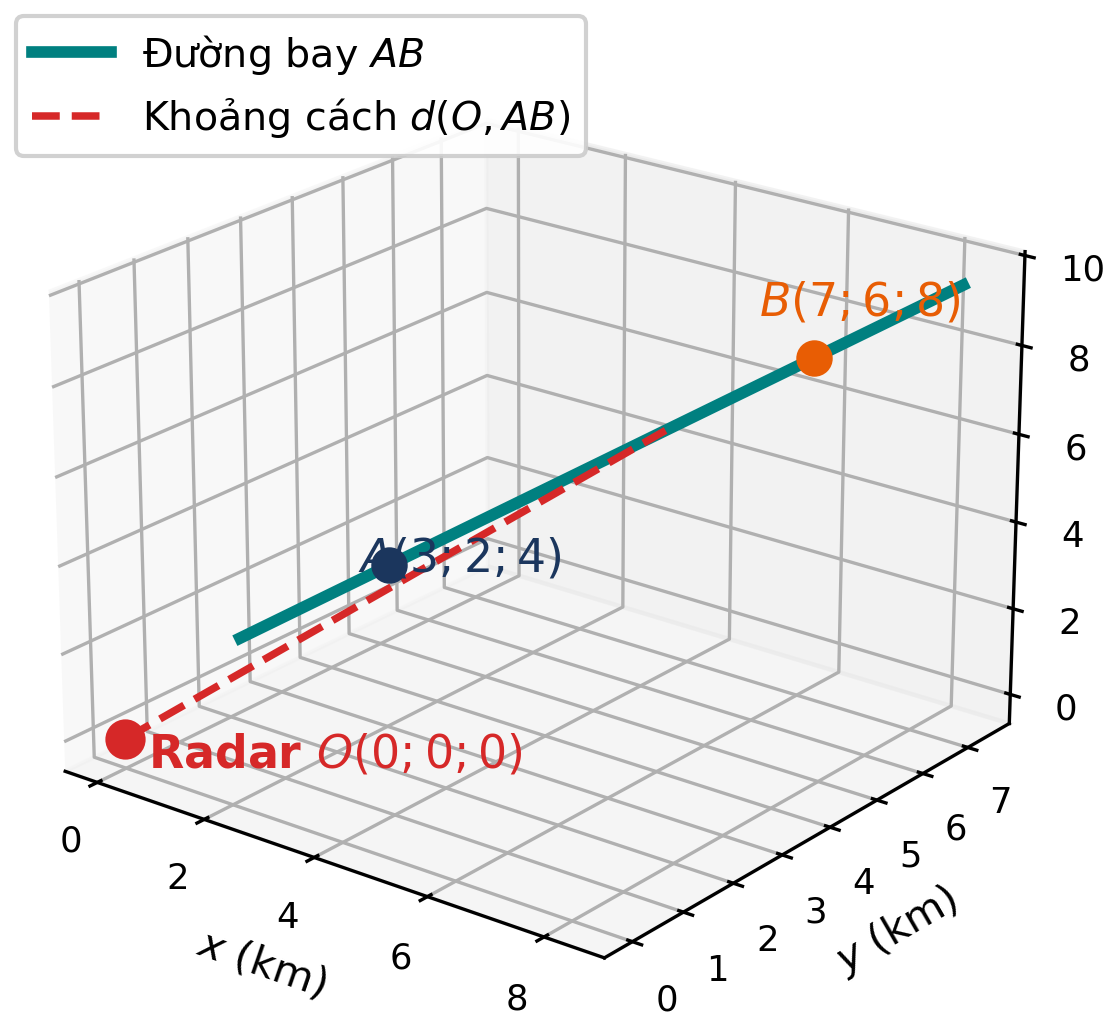
\includegraphics[width=\linewidth]{images/phan3_cau3_maybayradar.png}
\end{minipage}

\item Khảo sát mức thu nhập hàng tháng (đơn vị: triệu đồng) của $80$ công nhân tại một khu công nghiệp thu được bảng số liệu ghép nhóm sau:
\begin{center}
\begin{tabular}{|c|c|c|c|c|c|}
\hline
\textbf{Thu nhập (triệu đồng)} & $[6; 9)$ & $[9; 12)$ & $[12; 15)$ & $[15; 18)$ & $[18; 21)$ \\ \hline
\textbf{Số công nhân} & $12$ & $28$ & $24$ & $11$ & $5$ \\ \hline
\end{tabular}
\end{center}
Tính tứ phân vị thứ nhất $Q_1$ của mẫu số liệu ghép nhóm trên (làm tròn kết quả đến hàng phần mười).

\item Một xí nghiệp dệt may sử dụng 3 dây chuyền may tự động $A, B, C$ với tỉ lệ sản phẩm cung ứng lần lượt là $50\%$, $30\%$ và $20\%$. Tỉ lệ sản phẩm bị lỗi đường may do các chuyền $A, B, C$ tạo ra tương ứng là $2\%$, $3\%$ và $4\%$. Lấy ngẫu nhiên một sản phẩm trong kho hàng để kiểm tra. Tính xác suất để sản phẩm được chọn bị lỗi đường may (kết quả viết dưới dạng số thập phân).
\begin{center}
    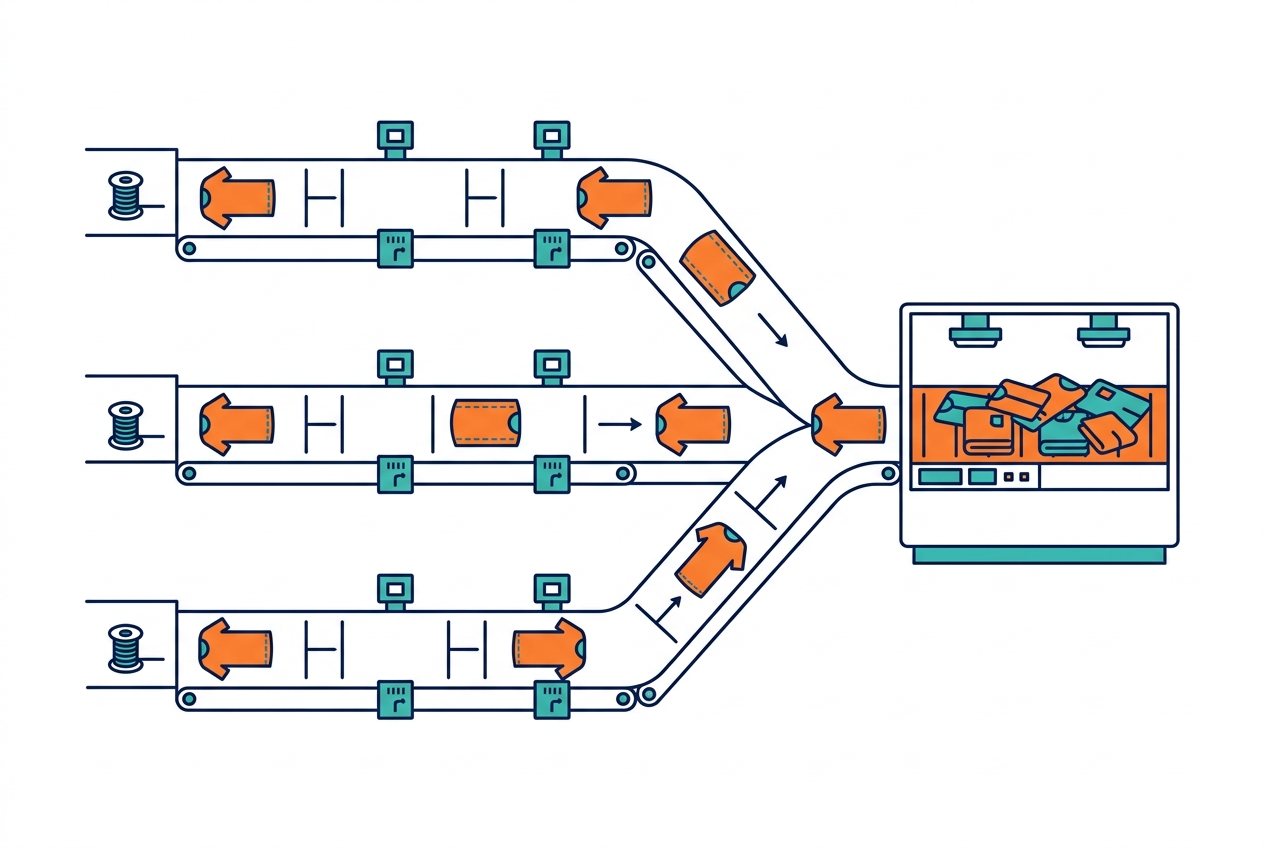
\includegraphics[width=0.42\linewidth,height=3.2cm,keepaspectratio]{images/phan3_cau5_daychuyenmay.jpg}
\end{center}

\item Hai bạn Hải và Sơn cùng chơi một trò chơi bốc bóng ngẫu nhiên. Hải có một hộp gồm 9 quả bóng được đánh số từ 1 đến 9. Sơn có một hộp gồm 8 quả bóng được đánh số từ 1 đến 8. Mỗi bạn bốc ngẫu nhiên 3 quả bóng từ hộp của mình, rồi xếp các số ghi trên 3 quả bóng bốc được theo thứ tự giảm dần để tạo thành một số có 3 chữ số. Bạn nào xếp được số lớn hơn là người chiến thắng. Tính xác suất để Sơn thua (làm tròn kết quả đến hàng phần trăm dưới dạng số thập phân).

\end{enumerate}

\newpage
% ==========================================
% BẢNG ĐÁP ÁN TỔNG HỢP
% ==========================================
\section*{BẢNG ĐÁP ÁN TỔNG HỢP}

\subsection*{1. PHẦN I}
\begin{center}
\begin{tabular}{|c|c||c|c||c|c||c|c|}
\hline
\textbf{Câu} & \textbf{Đáp án} & \textbf{Câu} & \textbf{Đáp án} & \textbf{Câu} & \textbf{Đáp án} & \textbf{Câu} & \textbf{Đáp án} \\ \hline
1 & C & 4 & C & 7 & D & 10 & C \\ \hline
2 & B & 5 & A & 8 & A & 11 & A \\ \hline
3 & D & 6 & B & 9 & B & 12 & D \\ \hline
\end{tabular}
\end{center}

\subsection*{2. PHẦN II}
\begin{center}
\begin{tabular}{|c|c|c|c|c|}
\hline
\textbf{Câu} & \textbf{Ý a)} & \textbf{Ý b)} & \textbf{Ý c)} & \textbf{Ý d)} \\ \hline
\textbf{1} & Đúng & Sai & Đúng & Đúng \\ \hline
\textbf{2} & Đúng & Sai & Đúng & Sai \\ \hline
\textbf{3} & Đúng & Đúng & Đúng & Sai \\ \hline
\textbf{4} & Đúng & Đúng & Đúng & Sai \\ \hline
\end{tabular}
\end{center}

\subsection*{3. PHẦN III}
\begin{center}
\begin{tabular}{|c|c||c|c||c|c|}
\hline
\textbf{Câu} & \textbf{Kết quả điền} & \textbf{Câu} & \textbf{Kết quả điền} & \textbf{Câu} & \textbf{Kết quả điền} \\ \hline
\textbf{1} & 0,6 & \textbf{3} & 1,4 & \textbf{5} & 0,027 \\ \hline
\textbf{2} & 44 & \textbf{4} & 9,9 & \textbf{6} & 0,66 \\ \hline
\end{tabular}
\end{center}

\newpage
% ==========================================
% HƯỚNG DẪN GIẢI CHI TIẾT
% ==========================================
\section*{HƯỚNG DẪN GIẢI CHI TIẾT}

\subsection*{PHẦN I}
\begin{enumerate}[label=\textbf{Câu \arabic*:}, leftmargin=*]
\item \textbf{Đáp án C.}
Ta có $y = \dfrac{x^2 - 3x + 6}{x - 1} = x - 2 + \dfrac{4}{x - 1}$.\\
Đạo hàm: $y' = 1 - \dfrac{4}{(x - 1)^2} = \dfrac{(x - 1)^2 - 4}{(x - 1)^2} = \dfrac{(x + 1)(x - 3)}{(x - 1)^2}$.\\
Cho $y' = 0 \iff x = -1$ hoặc $x = 3$.\\
Với $x = -1 \implies y(-1) = \dfrac{(-1)^2 - 3(-1) + 6}{-1 - 1} = -5 \implies A(-1; -5)$.\\
Với $x = 3 \implies y(3) = \dfrac{3^2 - 3(3) + 6}{3 - 1} = 3 \implies B(3; 3)$.\\
Khoảng cách giữa hai điểm cực trị $A$ và $B$ là:
$$AB = \sqrt{(3 - (-1))^2 + (3 - (-5))^2} = \sqrt{4^2 + 8^2} = \sqrt{16 + 64} = \sqrt{80} = 4\sqrt{5}.$$

\item \textbf{Đáp án B.}
Xét hàm số $C(t) = \dfrac{30t}{t^2 + 9}$ với $t \ge 0$.\\
Đạo hàm: $C'(t) = \dfrac{30(t^2 + 9) - 30t(2t)}{(t^2 + 9)^2} = \dfrac{30(9 - t^2)}{(t^2 + 9)^2}$.\\
Với $t \ge 0$, ta có $C'(t) = 0 \iff 9 - t^2 = 0 \iff t = 3$.\\
Bảng biến thiên cho thấy $C(t)$ đồng biến trên $(0; 3)$ và nghịch biến trên $(3; +\infty)$.\\
Do đó, nồng độ thuốc cao nhất đạt được tại thời điểm $t = 3\text{ giờ}$ với giá trị:
$$C_{\max} = C(3) = \dfrac{30(3)}{3^2 + 9} = \dfrac{90}{18} = 5\text{ mg/L}.$$

\item \textbf{Đáp án D.}
Bất phương trình $\log_{0{,}5}(x^2 - 4x + m) \ge -3 \iff 0 < x^2 - 4x + m \le (0{,}5)^{-3} = 8$.\\
Đặt $f(x) = x^2 - 4x$ trên đoạn $[1; 3]$. Ta có $f'(x) = 2x - 4 = 0 \iff x = 2 \in [1; 3]$.\\
Tính giá trị: $f(1) = -3$, $f(2) = -4$, $f(3) = -3$. Do đó trên $[1; 3]$ thì $\min f(x) = -4$ và $\max f(x) = -3$.\\
Để bất phương trình nghiệm đúng với mọi $x \in [1; 3]$, ta phải có:
$$\begin{cases} f(x) + m > 0 \\ f(x) + m \le 8 \end{cases} \iff \begin{cases} m > -\min_{[1; 3]} f(x) = 4 \\ m \le 8 - \max_{[1; 3]} f(x) = 11 \end{cases} \iff 4 < m \le 11.$$
Kết hợp với $m \in \mathbb{Z}$ và $m \in [-10; 10]$, ta được $m \in \{5; 6; 7; 8; 9; 10\}$.\\
Vậy có đúng $6$ giá trị nguyên của tham số $m$ thỏa mãn.

\item \textbf{Đáp án C.}
Công cơ học sinh ra là:
\begin{align*}
W &= \int_0^{0{,}5} (400x + 120x^2) dx = \left[ 200x^2 + 40x^3 \right]_0^{0{,}5} \\
&= 200(0{,}25) + 40(0{,}125) = 50 + 5 = 55\text{ J}.
\end{align*}

\item \textbf{Đáp án A.}
Mặt phẳng $(P)$ có vectơ pháp tuyến $\vec{n} = (2; -2; 1)$.\\
Đường thẳng $\Delta$ đi qua $A(2; 1; -3)$ và vuông góc với $(P)$ có phương trình tham số:
$$\begin{cases} x = 2 + 2t \\ y = 1 - 2t \\ z = -3 + t \end{cases}$$
Tọa độ hình chiếu vuông góc $H$ là giao điểm của $\Delta$ và $(P)$:
\begin{align*}
&2(2 + 2t) - 2(1 - 2t) + (-3 + t) - 8 = 0 \\
&\iff 9t - 9 = 0 \iff t = 1.
\end{align*}
Thay $t = 1$ vào phương trình tham số ta được tọa độ $H(4; -1; -2)$.

\item \textbf{Đáp án B.}
Cỡ mẫu $N = 8 + 16 + 14 + 8 + 4 = 50$.
\begin{itemize}[leftmargin=*]
    \item Tứ phân vị thứ nhất $Q_1$: $\dfrac{N}{4} = 12{,}5$. Nhóm 1 có tần số 8; nhóm 2 có tần số 16, tần số tích lũy là $24 \ge 12{,}5$. Do đó nhóm chứa $Q_1$ là nhóm $[10; 15)$:
    $$Q_1 = 10 + \dfrac{12{,}5 - 8}{16} \times (15 - 10) = 10 + \dfrac{22{,}5}{16} = 11{,}40625\text{ giờ}.$$
    \item Tứ phân vị thứ ba $Q_3$: $\dfrac{3N}{4} = 37{,}5$. Tích lũy trước nhóm 3 là $24$; nhóm 3 có tần số 14, tích lũy đến nhóm 3 là $38 \ge 37{,}5$. Do đó nhóm chứa $Q_3$ là $[15; 20)$:
    $$Q_3 = 15 + \dfrac{37{,}5 - 24}{14} \times (20 - 15) = 15 + \dfrac{67{,}5}{14} \approx 19{,}8214\text{ giờ}.$$
\end{itemize}
Khoảng tứ phân vị:
$$\Delta_Q = Q_3 - Q_1 \approx 19{,}8214 - 11{,}40625 = 8{,}41515 \approx 8{,}42\text{ giờ}.$$

\item \textbf{Đáp án D.}
Theo công thức cộng xác suất:
$$P(A \cap B) = P(A) + P(B) - P(A \cup B) = 0{,}65 + 0{,}50 - 0{,}85 = 0{,}30.$$
Xác suất có điều kiện học sinh thích môn Bóng rổ khi biết học sinh đó thích môn Bóng đá là:
$$P(B|A) = \dfrac{P(A \cap B)}{P(A)} = \dfrac{0{,}30}{0{,}65} = \dfrac{6}{13} \approx 0{,}4615 \approx 0{,}46.$$

\item \textbf{Đáp án A.}
Chia đa thức: $2x^2 + 3x - 1 = (2x - 1)(x + 2) + 1 \implies y = 2x - 1 + \dfrac{1}{x + 2}$.\\
Vì $\lim\limits_{x \to \pm\infty} \left[ y - (2x - 1) \right] = \lim\limits_{x \to \pm\infty} \dfrac{1}{x + 2} = 0$, nên đường thẳng $d: y = 2x - 1$ là tiệm cận xiên của đồ thị hàm số.\\
Tìm giao điểm của $d$ với hai trục tọa độ:
\begin{itemize}
    \item Với $Ox$ ($y = 0$): $2x - 1 = 0 \iff x = \dfrac{1}{2} \implies M\left(\dfrac{1}{2}; 0\right) \implies OM = \dfrac{1}{2}$.
    \item Với $Oy$ ($x = 0$): $y = -1 \implies N(0; -1) \implies ON = 1$.
\end{itemize}
Diện tích tam giác $OMN$ vuông tại $O$ là:
$$S = \dfrac{1}{2} OM \cdot ON = \dfrac{1}{2} \times \dfrac{1}{2} \times 1 = \dfrac{1}{4} = 0{,}25.$$

\item \textbf{Đáp án B.}
Sau thời gian $t$ ngày, khối lượng I-ốt 131 còn lại là $m(t) = m_0 \cdot \left(\dfrac{1}{2}\right)^{t / T}$ với $m_0 = 200\text{ mg}$ và chu kỳ $T = 8\text{ ngày}$.\\
Với $t = 32\text{ ngày}$, số chu kỳ bán rã là $\dfrac{32}{8} = 4$.\\
Khối lượng còn lại là:
$$m(32) = 200 \times \left(\dfrac{1}{2}\right)^4 = \dfrac{200}{16} = 12{,}5\text{ mg}.$$

\item \textbf{Đáp án C.}
Mặt cầu $(S)$ có tâm $I(1; 2; -1)$ và bán kính $R = \sqrt{9} = 3$.\\
Khoảng cách từ tâm $I$ đến điểm $A$ là:
$$IA = \sqrt{(4 - 1)^2 + (6 - 2)^2 + (11 - (-1))^2} = \sqrt{3^2 + 4^2 + 12^2} = \sqrt{169} = 13.$$
Vì $IA = 13 > R = 3$, nên điểm $A$ nằm ngoài mặt cầu $(S)$.\\
Khoảng cách ngắn nhất từ $A$ đến một điểm $M$ bất kỳ trên mặt cầu là:
$$d_{\min} = IA - R = 13 - 3 = 10.$$

\item \textbf{Đáp án A.}
Phương trình hoành độ giao điểm của đồ thị hàm số với trục $Ox$:
$$\sqrt{x \ln x} = 0 \iff x \ln x = 0 \iff x = 1\quad (\text{do điều kiện } x > 0 \text{ và } \ln x \ge 0 \implies x \ge 1).$$
Thể tích khối tròn xoay tạo thành khi quay quanh $Ox$ là:
$$V = \pi \int_1^e \left(\sqrt{x \ln x}\right)^2 dx = \pi \int_1^e x \ln x dx.$$
Đặt $\begin{cases} u = \ln x \\ dv = x dx \end{cases} \implies \begin{cases} du = \dfrac{1}{x} dx \\ v = \dfrac{x^2}{2} \end{cases}$.\\
Áp dụng công thức tích phân từng phần:
\begin{align*}
\int_1^e x \ln x dx &= \left[ \dfrac{x^2}{2} \ln x \right]_1^e - \dfrac{1}{2} \int_1^e x dx \\
&= \dfrac{e^2}{2} - \left[ \dfrac{x^2}{4} \right]_1^e = \dfrac{e^2}{2} - \left(\dfrac{e^2}{4} - \dfrac{1}{4}\right) = \dfrac{e^2 + 1}{4}.
\end{align*}
Vậy thể tích $V = \dfrac{\pi(e^2 + 1)}{4}$.

\item \textbf{Đáp án D.}
Đạo hàm: $y' = 3x^2 - 6mx + 3(m^2 - 1) = 3\left[ x^2 - 2mx + m^2 - 1 \right]$.\\
Xét phương trình $y' = 0 \iff g(x) = x^2 - 2mx + m^2 - 1 = 0$.\\
Ta có $\Delta' = m^2 - (m^2 - 1) = 1 > 0$ với mọi $m \in \mathbb{R}$. Do đó hàm số luôn có 2 điểm cực trị $x_1, x_2$ phân biệt với mọi $m$.\\
Theo định lý Vi-ét: $\begin{cases} x_1 + x_2 = 2m \\ x_1 x_2 = m^2 - 1 \end{cases}$.\\
Theo bài ra:
\begin{align*}
x_1^2 + x_2^2 &= (x_1 + x_2)^2 - 2x_1 x_2 = 4m^2 - 2(m^2 - 1) = 2m^2 + 2 = 10 \\
&\iff 2m^2 = 8 \iff m^2 = 4 \iff m = \pm 2.
\end{align*}
Cả hai giá trị $m = 2$ và $m = -2$ đều nguyên và thuộc $[-10; 10]$. Vậy có đúng 2 giá trị $m$ thỏa mãn.
\end{enumerate}

\subsection*{PHẦN II}
\begin{enumerate}[label=\textbf{Câu \arabic*:}, leftmargin=*]
\item \textbf{Câu 1 (Kinh tế xưởng may bảo hộ lao động):}
\begin{itemize}
    \item a) \textbf{Đúng}: Doanh thu bán $x$ trăm bộ là $R(x) = x \cdot p(x) = x(180 - 6x) = 180x - 6x^2$ (triệu đồng).
    \item b) \textbf{Sai}: Lợi nhuận $L(x) = R(x) - C(x) = (180x - 6x^2) - (x^3 - 18x^2 + 120x + 80) = -x^3 + 12x^2 + 60x - 80$ (triệu đồng). Phương án ghi $+80$ là sai dấu hệ số tự do.
    \item c) \textbf{Đúng}: Đạo hàm $L'(x) = -3x^2 + 24x + 60 = -3(x^2 - 8x - 20) = -3(x - 10)(x + 2)$.\\
    Với $0 < x \le 30$, ta có $L'(x) = 0 \iff x = 10$. Bảng biến thiên cho thấy hàm đạt cực đại tại $x = 10$, tương ứng với sản xuất $10$ trăm bộ ($1.000$ bộ).
    \item d) \textbf{Đúng}: Mức lợi nhuận cực đại đạt được là $L(10) = -(10)^3 + 12(10)^2 + 60(10) - 80 = -1000 + 1200 + 600 - 80 = 720$ triệu đồng.
\end{itemize}

\item \textbf{Câu 2 (Chuyển động ô tô điện phanh gấp):}
\begin{itemize}
    \item a) \textbf{Đúng}: Vận tốc của xe là $v(t) = v_0 + \int_0^t a(u) du = 27 + \int_0^t (-1{,}5u) du = 27 - 0{,}75t^2\text{ (m/s)}$.\\
    Tại $t = 2\text{ s}$, vận tốc là $v(2) = 27 - 0{,}75(4) = 27 - 3 = 24\text{ m/s}$.
    \item b) \textbf{Sai}: Gia tốc hãm tại $t = 4\text{ s}$ là $a(4) = -1{,}5(4) = -6\text{ m/s}^2 \implies$ độ lớn gia tốc là $6\text{ m/s}^2 \ne 5\text{ m/s}^2$.
    \item c) \textbf{Đúng}: Xe dừng lại hoàn toàn khi $v(t) = 0 \iff 27 - 0{,}75t^2 = 0 \iff t^2 = 36 \iff t = 6\text{ giây}$.
    \item d) \textbf{Sai}: Quãng đường xe di chuyển từ lúc phanh đến khi dừng hẳn là:
    \begin{align*}
    S &= \int_0^6 v(t) dt = \int_0^6 (27 - 0{,}75t^2) dt \\
    &= \left[ 27t - 0{,}25t^3 \right]_0^6 = 27(6) - 0{,}25(216) = 108\text{ m} < 110\text{ m}.
    \end{align*}
\end{itemize}

\item \textbf{Câu 3 (Tầm soát vi-rút cúm gia cầm):}
Gọi $N$ là biến cố ``Gia cầm bị nhiễm vi-rút'' và $D$ là biến cố ``Kết quả xét nghiệm dương tính''.\\
Theo giả thiết: $P(N) = 0{,}05$, do đó $P(\overline{N}) = 1 - 0{,}05 = 0{,}95$.\\
Độ nhạy $96\% \implies P(D|N) = 0{,}96$; độ đặc hiệu $90\% \implies P(\overline{D}|\overline{N}) = 0{,}90$.
\begin{itemize}
    \item a) \textbf{Đúng}: Xác suất con gia cầm không bị nhiễm vi-rút là $P(\overline{N}) = 0{,}95$.
    \item b) \textbf{Đúng}: Tỉ lệ dương tính giả là $P(D|\overline{N}) = 1 - P(\overline{D}|\overline{N}) = 1 - 0{,}90 = 0{,}10$.
    \item c) \textbf{Đúng}: Theo công thức xác suất toàn phần:
    \begin{align*}
    P(D) &= P(N) \cdot P(D|N) + P(\overline{N}) \cdot P(D|\overline{N}) \\
    &= 0{,}05 \times 0{,}96 + 0{,}95 \times 0{,}10 = 0{,}048 + 0{,}095 = 0{,}143.
    \end{align*}
    \item d) \textbf{Sai}: Theo công thức Bayes, xác suất gia cầm thực sự nhiễm vi-rút khi có kết quả dương tính là:
    $$P(N|D) = \dfrac{P(N \cap D)}{P(D)} = \dfrac{0{,}05 \times 0{,}96}{0{,}143} = \dfrac{0{,}048}{0{,}143} = \dfrac{48}{143} \approx 0{,}3357 = 33{,}57\% < 35\%.$$
\end{itemize}

\item \textbf{Câu 4 (Mái che vòm thép sân tennis Oxyz):}
\begin{itemize}
    \item a) \textbf{Đúng}: Vì mặt sàn nằm trên mặt phẳng $z = 0$, hình chiếu vuông góc của đỉnh $S(4; 5; 8)$ lên mặt sàn là điểm $H(4; 5; 0)$.
    \item b) \textbf{Đúng}: Chân cột $A(0; 0; 0)$ nên:
    $$SA = \sqrt{(4 - 0)^2 + (5 - 0)^2 + (8 - 0)^2} = \sqrt{16 + 25 + 64} = \sqrt{105}\text{ m}.$$
    \item c) \textbf{Đúng}: Tọa độ trọng tâm $G$ của tam giác $ABC$ với $A(0; 0; 0), B(8; 0; 0), C(8; 10; 0)$ là:
    $$x_G = \dfrac{0 + 8 + 8}{3} = \dfrac{16}{3},\quad y_G = \dfrac{0 + 0 + 10}{3} = \dfrac{10}{3},\quad z_G = 0 \implies G\left(\dfrac{16}{3}; \dfrac{10}{3}; 0\right).$$
    \item d) \textbf{Sai}: Hình chiếu vuông góc của đoạn thẳng $SA$ lên mặt sàn $(ABCD)$ là $HA$.\\
    Ta có $HA = \sqrt{(4 - 0)^2 + (5 - 0)^2} = \sqrt{16 + 25} = \sqrt{41}\text{ m}$ và $SH = 8\text{ m}$.\\
    Gọi $\alpha$ là góc giữa $SA$ và mặt sàn, ta có $\tan\alpha = \dfrac{SH}{HA} = \dfrac{8}{\sqrt{41}} \approx \dfrac{8}{6{,}403} \approx 1{,}249 > 1 = \tan 45^\circ \implies \alpha \approx 51{,}32^\circ > 45^\circ$.
\end{itemize}

\end{enumerate}

\subsection*{PHẦN III}
\begin{enumerate}[label=\textbf{Câu \arabic*:}, leftmargin=*]
\item \textbf{Đáp số: 0,6.}
Thể tích thùng rác hình hộp chữ nhật không nắp có đáy hình vuông cạnh $x$ và chiều cao $h$ là:
$$V = x^2 h = 0{,}162 \implies h = \dfrac{0{,}162}{x^2}\text{ (m)}.$$
Diện tích đáy là $S_{\text{đáy}} = x^2\text{ (m}^2\text{)}$; diện tích 4 mặt bên là $S_{\text{xq}} = 4xh = 4x \cdot \dfrac{0{,}162}{x^2} = \dfrac{0{,}648}{x}\text{ (m}^2\text{)}$.\\
Tổng chi phí làm thùng bằng tôn là:
$$C(x) = 150000 \cdot x^2 + 100000 \cdot \dfrac{0{,}648}{x} = 150000x^2 + \dfrac{64800}{x}\quad (x > 0).$$
Đạo hàm:
$$C'(x) = 300000x - \dfrac{64800}{x^2} = \dfrac{300000x^3 - 64800}{x^2}.$$
Cho $C'(x) = 0 \iff 300000x^3 = 64800 \iff x^3 = \dfrac{64800}{300000} = 0{,}216 \iff x = \sqrt[3]{0{,}216} = 0{,}6\text{ m}$.\\
Bảng biến thiên cho thấy $C(x)$ đạt giá trị nhỏ nhất tại $x = 0{,}6\text{ m}$.\\
Đáp số điền: \textbf{0,6}.

\item \textbf{Đáp số: 44.}
Số tiền gửi định kỳ mỗi tháng là $A = 10$ triệu đồng, lãi suất $r = 0{,}6\% = 0{,}006$/tháng.\\
Số tiền tích lũy sau $n$ tháng theo hình thức gửi đầu mỗi tháng là:
$$S_n = A(1 + r) \cdot \dfrac{(1 + r)^n - 1}{r} = 10(1{,}006) \cdot \dfrac{(1{,}006)^n - 1}{0{,}006} = \dfrac{10{,}06}{0{,}006} \left[(1{,}006)^n - 1\right].$$
Yêu cầu $S_n \ge 500$:
$$\dfrac{10{,}06}{0{,}006} \left[(1{,}006)^n - 1\right] \ge 500 \iff (1{,}006)^n - 1 \ge \dfrac{500 \times 0{,}006}{10{,}06} = \dfrac{3}{10{,}06} \approx 0{,}29821$$
$$\iff (1{,}006)^n \ge 1{,}29821 \iff n \ge \dfrac{\ln(1{,}29821)}{\ln(1{,}006)} \approx \dfrac{0{,}26098}{0{,}005982} \approx 43{,}628.$$
Vì số tháng $n$ là số nguyên nên chị Mai cần gửi liên tục ít nhất $44$ tháng.\\
Đáp số điền: \textbf{44}.

\item \textbf{Đáp số: 1,4.}
Vectơ chỉ phương của đường bay đi qua $A(3; 2; 4)$ và $B(7; 6; 8)$ là:
$$\overrightarrow{AB} = (4; 4; 4) = 4(1; 1; 1) \implies \vec{u} = (1; 1; 1).$$
Vectơ vị trí từ đài ra-đa $O(0; 0; 0)$ đến mốc $A$ là $\overrightarrow{OA} = (3; 2; 4)$.\\
Tích có hướng:
$$\left[ \overrightarrow{OA}, \vec{u} \right] = (2 \cdot 1 - 4 \cdot 1;\; 4 \cdot 1 - 3 \cdot 1;\; 3 \cdot 1 - 2 \cdot 1) = (-2; 1; 1).$$
Độ dài: $\left| \left[ \overrightarrow{OA}, \vec{u} \right] \right| = \sqrt{(-2)^2 + 1^2 + 1^2} = \sqrt{6}$; độ dài $|\vec{u}| = \sqrt{1^2 + 1^2 + 1^2} = \sqrt{3}$.\\
Khoảng cách ngắn nhất từ đài ra-đa $O$ đến đường bay là:
$$d(O, AB) = \dfrac{\left| \left[ \overrightarrow{OA}, \vec{u} \right] \right|}{|\vec{u}|} = \dfrac{\sqrt{6}}{\sqrt{3}} = \sqrt{2} \approx 1{,}4142 \approx 1{,}4\text{ km}.$$
Đáp số điền: \textbf{1,4}.

\item \textbf{Đáp số: 9,9.}
Tổng số công nhân là $N = 12 + 28 + 24 + 11 + 5 = 80$.\\
Ta có $\dfrac{N}{4} = \dfrac{80}{4} = 20$.\\
Tần số tích lũy của nhóm thứ nhất $[6; 9)$ là $12 < 20$.\\
Tần số tích lũy của nhóm thứ hai $[9; 12)$ là $12 + 28 = 40 \ge 20$.\\
Do đó, nhóm chứa tứ phân vị thứ nhất $Q_1$ là nhóm $[9; 12)$, với đầu mút dưới $L = 9$, độ dài nhóm $h = 12 - 9 = 3$, tần số nhóm $n_2 = 28$, và tần số tích lũy của nhóm trước là $C = 12$.\\
Áp dụng công thức:
$$Q_1 = L + \dfrac{\dfrac{N}{4} - C}{n_2} \cdot h = 9 + \dfrac{20 - 12}{28} \cdot 3 = 9 + \dfrac{24}{28} = 9 + \dfrac{6}{7} \approx 9{,}8571 \approx 9{,}9\text{ triệu đồng}.$$
Đáp số điền: \textbf{9,9}.

\item \textbf{Đáp số: 0,027.}
Gọi $A, B, C$ lần lượt là biến cố sản phẩm được may bởi chuyền $A$, chuyền $B$, chuyền $C$.\\
Theo bài ra: $P(A) = 0{,}50$; $P(B) = 0{,}30$; $P(C) = 0{,}20$ với $P(A) + P(B) + P(C) = 1$.\\
Gọi $L$ là biến cố ``Sản phẩm lấy ra bị lỗi đường may''.\\
Theo giả thiết: $P(L|A) = 0{,}02$; $P(L|B) = 0{,}03$; $P(L|C) = 0{,}04$.\\
Theo công thức xác suất toàn phần:
$$P(L) = P(A) \cdot P(L|A) + P(B) \cdot P(L|B) + P(C) \cdot P(L|C)$$
$$= 0{,}50 \times 0{,}02 + 0{,}30 \times 0{,}03 + 0{,}20 \times 0{,}04 = 0{,}010 + 0{,}009 + 0{,}008 = 0{,}027.$$
Đáp số điền: \textbf{0,027}.

\item \textbf{Đáp số: 0,66.}
Số cách bốc 3 quả bóng của Hải từ 9 quả bóng là $C_9^3 = 84$.\\
Số cách bốc 3 quả bóng của Sơn từ 8 quả bóng là $C_8^3 = 56$.\\
Số phần tử của không gian mẫu là $|\Omega| = C_9^3 \times C_8^3 = 84 \times 56 = 4704$.\\
Khi bốc được 3 quả bóng, mỗi bạn chỉ có duy nhất một cách sắp xếp các chữ số theo thứ tự giảm dần để tạo thành một số có 3 chữ số.\\
Do đó, việc bạn nào tạo được số lớn hơn hoàn toàn tương đương với việc so sánh hai tập hợp gồm 3 phần tử được bốc.\\
Ta xét hai trường hợp đối với kết quả bốc của Hải:
\begin{itemize}
    \item \textbf{Trường hợp 1}: Hải bốc được quả bóng mang số 9.\\
    Số cách chọn của Hải là $C_1^1 \times C_8^2 = 28$ cách.\\
    Vì hộp của Sơn chỉ gồm các bóng từ 1 đến 8 nên số của Sơn có chữ số hàng trăm lớn nhất chỉ có thể là 8, trong khi số của Hải có chữ số hàng trăm là 9. Do đó trong mọi kết quả ở trường hợp này Hải luôn thắng (tức Sơn thua).\\
    Số kết quả thuận lợi trong trường hợp này là: $28 \times C_8^3 = 28 \times 56 = 1568$.
    
    \item \textbf{Trường hợp 2}: Hải không bốc được quả bóng mang số 9.\\
    Nghĩa là cả 3 quả bóng của Hải đều được bốc từ tập $\{1; 2; \dots; 8\}$. Số cách bốc của Hải là $C_8^3 = 56$ cách.\\
    Trong trường hợp này, cả Hải và Sơn đều độc lập chọn ra 3 số từ cùng một tập 8 số $\{1; 2; \dots; 8\}$.\\
    Tổng số cặp kết quả là $56 \times 56 = 3136$.\\
    Trong đó, hai bạn hòa nhau khi và chỉ khi cùng chọn ra một bộ 3 số giống hệt nhau, có $C_8^3 = 56$ kết quả hòa.\\
    Do tính đối xứng hoàn toàn giữa Hải và Sơn, số trường hợp Hải thắng bằng số trường hợp Sơn thắng và bằng:
    $$\dfrac{3136 - 56}{2} = 1540\text{ trường hợp}.$$
\end{itemize}
Tổng số trường hợp Sơn thua (tức Hải thắng) là:
$$N = 1568 + 1540 = 3108\text{ trường hợp}.$$
Xác suất để Sơn thua là:
$$P = \dfrac{3108}{4704} = \dfrac{37}{56} \approx 0{,}6607 \approx 0{,}66.$$
Đáp số điền: \textbf{0,66}.
\end{enumerate}

\end{document}
